% 第 17 题多面体（平行四边形 ABCD 上立平面 AED，含 F、E 与 BC 中点 G）：
% 按固定源 PDF 矢量路径端点换算（1 pt → 0.03515 cm）；原点取 C 点，y 向上。
% 源页顶点 pt：E(391.63,174.74)、F(334.74,174.74)、A(344.37,320.41)、B(230.60,320.41)、
% C(184.85,337.27)、D(298.62,337.27)、G(207.73,328.84)（G 为 BC 中点，坐标精确吻合）。
% 实线 6 条：EF、FC、CD、DA、DE、AE；虚线 6 条：CB、BA、BD、GF、BF、BE。先画虚线后画实线。
% 注：该图为示意，不按题设比例（∠BAD 实测约 20°、AB:BC 实测约 2.33:1），照源描摹，不按数值重定比例。
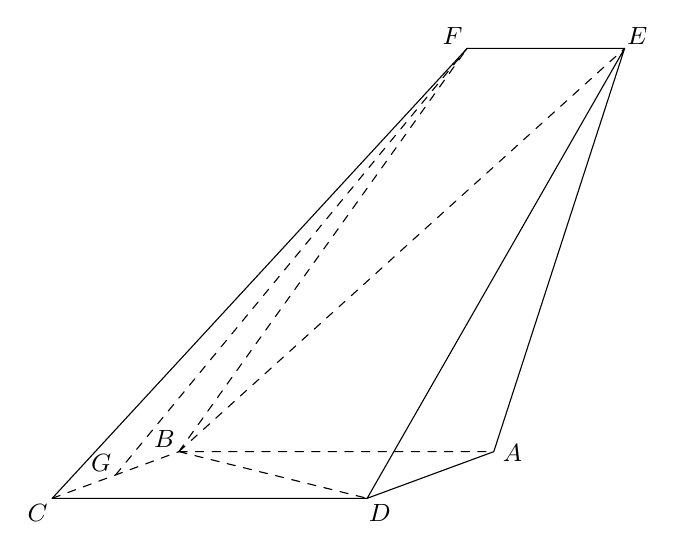
\begin{tikzpicture}[line cap=round,line join=round,font=\small,x=0.03515cm,y=0.03515cm]
\coordinate (E) at (206.78,162.53);
\coordinate (F) at (149.89,162.53);
\coordinate (A) at (159.52,16.86);
\coordinate (B) at (45.75,16.86);
\coordinate (C) at (0,0);
\coordinate (D) at (113.77,0);
\coordinate (G) at (22.88,8.43);
% 虚线先画（标签用 inner sep=0 + 源字形左端/基线显式坐标：TikZ 节点默认 inner sep
% 0.3333em 会把字形右移约 3pt，令 B/G 贴入顶点虚线簇；本图经 400 dpi 隔离探头
% 8-连通域验证 7 字母均为独立分量）
\draw[dashed] (C)--(B);
\draw[dashed] (B)--(A) (B)--(D) (G)--(F) (B)--(F) (B)--(E);
% 实线后画
\draw (E)--(F) (F)--(C) (C)--(D) (D)--(A) (D)--(E) (A)--(E);
% 标注（显式坐标：源字形左端与基线换算；不并入线段）
\node[anchor=base west,inner sep=0] at (140.86,163.87) {$F$};
\node[anchor=base west,inner sep=0] at (207.53,163.87) {$E$};
\node[anchor=base west,inner sep=0] at (162.56,13.27) {$A$};
\node[anchor=base west,inner sep=0] at (36.58,18.20) {$B$};
\node[anchor=base west,inner sep=0] at (13.82,9.77) {$G$};
\node[anchor=base west,inner sep=0] at (-9.06,-8.52) {$C$};
\node[anchor=base west,inner sep=0] at (114.21,-8.52) {$D$};
\end{tikzpicture}
